\section{Generalized Critic Policy Optimization}
\label{sec:method}

In this section, we will present our proposed theoretical model, which we call the Generalized Critic. We start by giving a visual representation with an illustrative example to establish the intuition behind this practical view. We then move on to a more technical definition of each element.

For our practical case, we consider the case of an infinite horizon MDP. The set of actions $\mathcal{A}$ and the set of states $\mathcal{S}$ are continuous. $\pi_\theta$, the estimated policy with parameters $\theta$, is a gaussian probability distribution.

Let us consider the following scenario of a policy update: 
at epoch $k+1$, the current policy $\pi_{\theta_k}$ is used to sample training data from the environment through a cycle of actions ($a_t$) and feedback (the next state $s_{t+1}$, and the reward $r_t$). This execution scenario starting from the initial state $s_0$ up to the final state is called an \emph{episode}. The set of all states, actions and rewards the agent has experienced in an episode is called a \emph{trajectory}. 

The training sample of each epoch is a set $\mathcal{D}_k$ containig a given number of trajectories; in implementations, this corresponds to the minibatch for each update. The critic will update the estimator $\hat{V}(s_t)$ based on the new data, after which the advantage function is estimated. Following that, the policy update is performed, guided by the advantage function. There are several methods to optimize the policy gradient, so the specifics of this update will depend on the used algorithm.

We bring two additions to the standard scenario as shown in figure \ref{fig:model}.

\subsection{Generalized Critic}

%scénario d'exécution ici
% puis faire une sous-section pour expliquer la fonction et le fonctionnement du modèle
% puis parler d'espace d'action continu et gaussian distribution dans experiments

The generalized critic is a substitute for the critic in the standard actor-critic view. It computes one or more estimations for either or both of the value function $\hat{V}(s_t)$ and the corresponding advantage function $\hat{A}(a_t, s_t)$. The difference in the estimations may reside in one or more of the following points:
\begin{itemize}
\item Network architecture
\item Scalar factors values
\item Methods of estimation
\end{itemize}

As empirical data in other data science applications suggest \cite{xiao2018deep}, combining different methods when approximating a function often yields superior estimations as a result of a smaller variance in results. In the particular context of deep reinforcement learning, hyperparameters such as scalar factor values, network architectures and other implementation details have been shown to have drastic influence on the learning process and reported results \cite{islam2017reproducibility}. Thus, we assume that combining models with as little as a change in hyperparameter values has potential to improve the final estimation.

\begin{figure}[!htb]
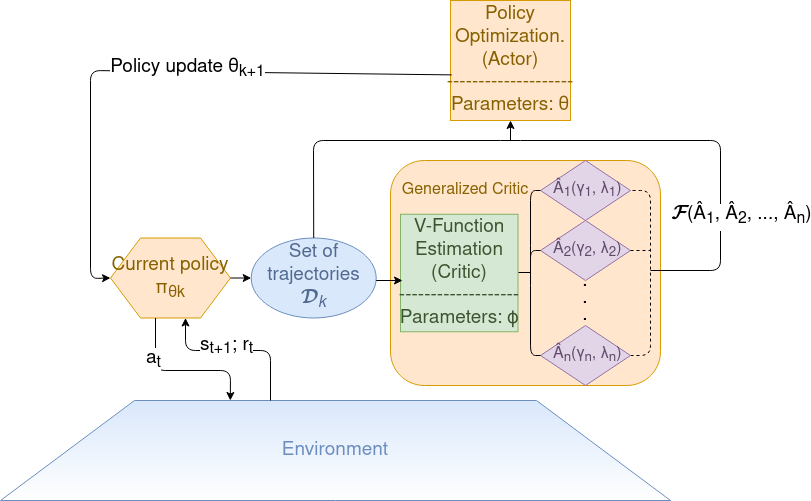
\includegraphics[width=8.5cm]{images/model}
\caption{Policy update scenario with a generalized critic.}
\label{fig:model}
\end{figure}

\subsection{The Aggregation Function}

Out of the possible estimations of the advantage function, a final value is ultimately needed to perform the policy update. However, the accuracy of different estimates is not known in advance, and in all likeliness, varies at different steps of the policy update. We would like a method to automatically select, or deduce an advantage value for the current epoch. Ideally, this would help automatically and adaptively adjust the critic's final value towards a more accurate estimation during the policy training.

For that sake, we included in our theoretical model a function $\mathcal{F}: \mathbb{R}^n \mapsto \mathbb{R}$, which we call straightforwardly the aggregation function. 

The aggregation function takes any number of critic values as input and outputs a single value to be used in the policy update. The function itself could be defined at implementation,  or trained to optimize the policy gradient. The estimated parameters would be updated dynamically as the policy gradient estimate changes.
